\section{Deep Speed Inference}
\begin{frame}{DeepSpeed Inference: Optimized Kernels}
\textbf{Challenges}: small batch size leads to limited work in kernels

\begin{enumerate}
    \setlength{\itemsep}{.5pt}
    \item The overheads associated with kernel invocation become significant. $\rightarrow$ \textcolor{byzantium}{\hl{Kernel fusion}}
    \item The performance is limited by the memory bandwidth utilization in reading weights. $\rightarrow$ \textcolor{byzantium}{\hl{Data reuse at shared memory or regiter level}}
    \item Both CuTLASS and CuBLAS are not well-optimized for small batch size.  $\rightarrow$ \textcolor{byzantium}{\hl{Optimize GEMM kernels for small matrix sizes}}
\end{enumerate}

\end{frame}

\begin{frame}{DeepSpeed Inference: SBI-GeMM}
    \begin{figure}
        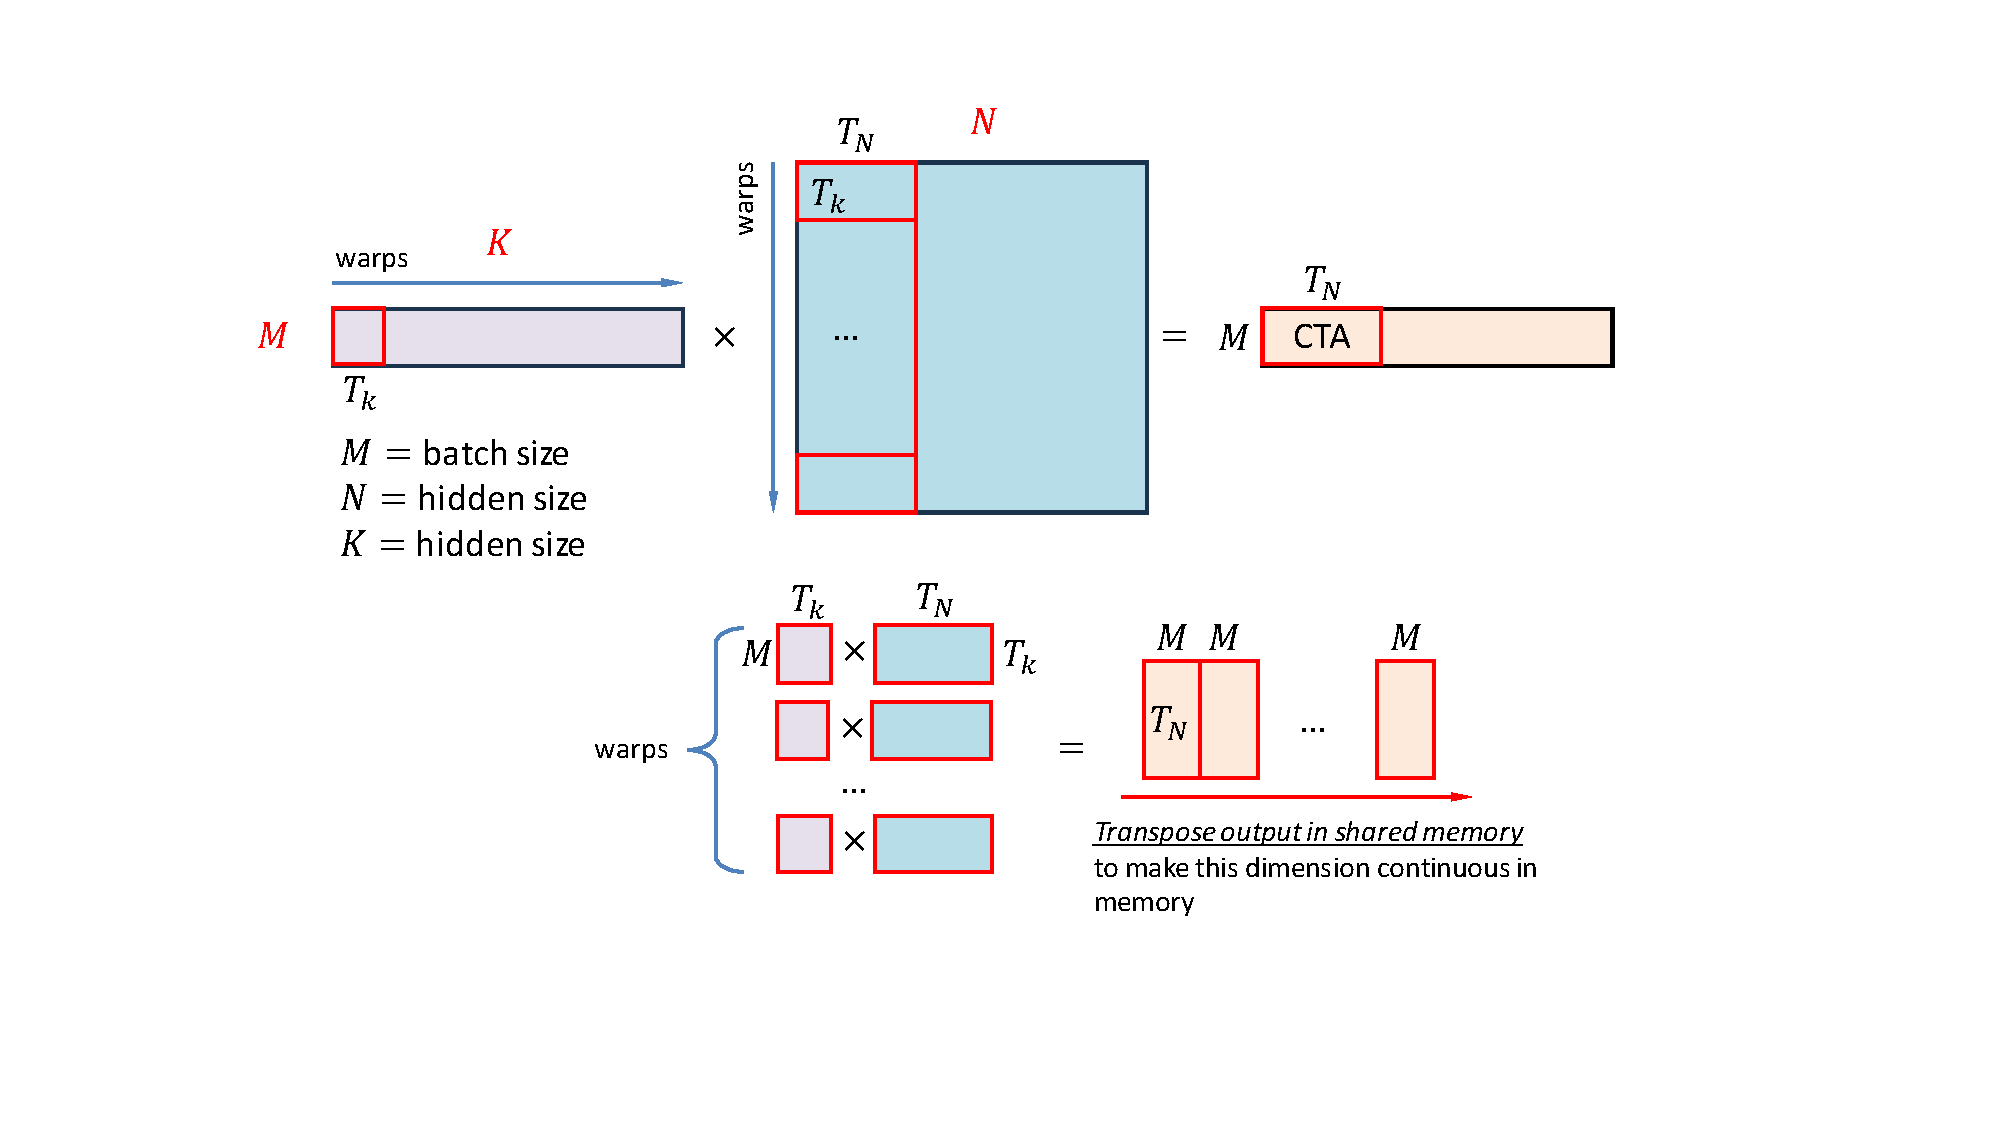
\includegraphics[width=0.75\linewidth]{./images/SBI-GEMM.pdf}
        \caption{Rationale of the SBI-GeMM}
    \end{figure}
    \footnotesize{
    \begin{enumerate}
        \item \hl{tile strategies}: tile dimensionality $N$ first, if this does not produce enough parallelism, tile $K$ then.
        \item \hl{cooperative-group reduction}: transpose output tile on the shared memory
        \item \hl{leverage full cache-line}.
    \end{enumerate}
    }
\end{frame}

\begin{frame}{DeepSpeed Inference: Fused Transformer Block}
    \begin{figure}
        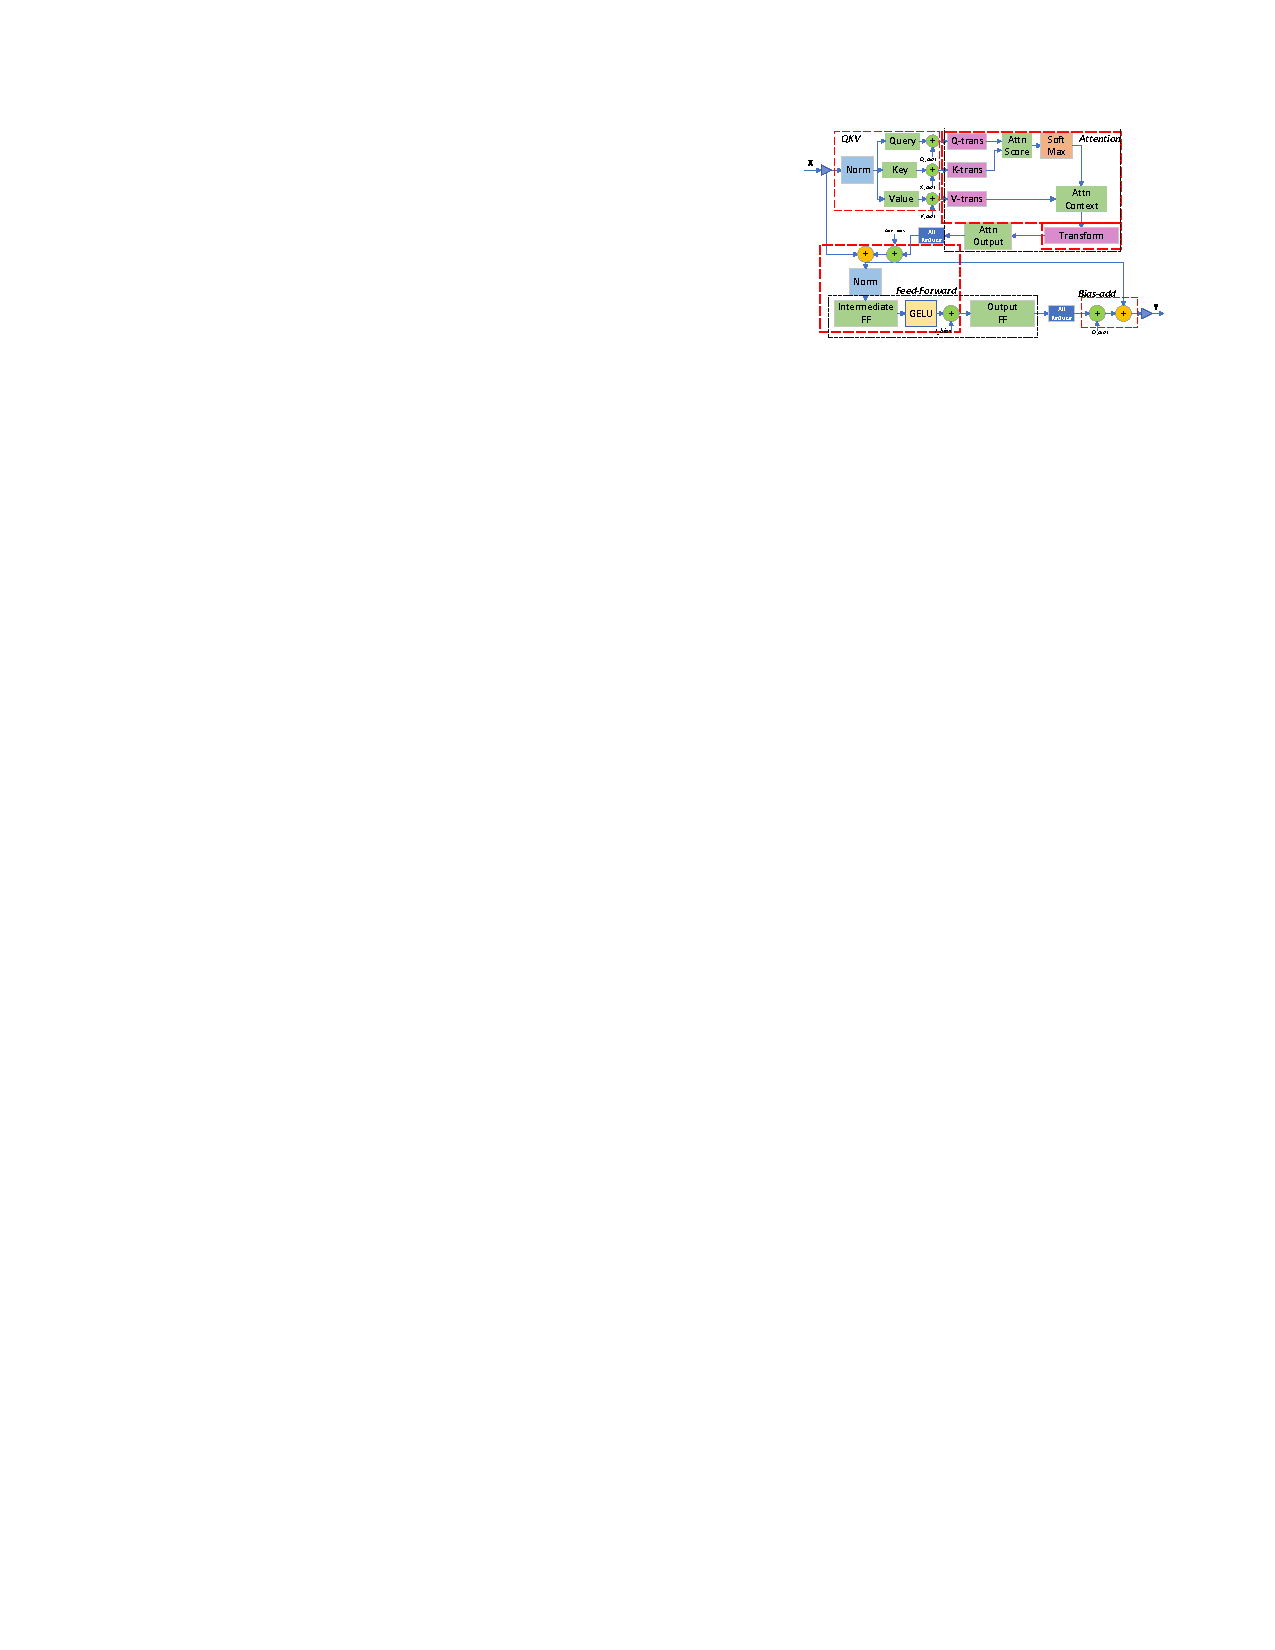
\includegraphics[width=0.85\linewidth]{./images/fused_transformer_block-deepspeed-inference.pdf}
        \caption{Fusion regions in DeepSpeed inference.}
    \end{figure}
    \footnotesize{
    \begin{enumerate}
        \item[] \hl{large-batch transformer}: use CuBLAS for GEMM and keep GEMMs unfused.
    \end{enumerate}
    }
\end{frame}

\begin{frame}{DeepSpeed Inference: Inference on Many GPU System: I}
    \center\textbf{Goals}
    \begin{enumerate}
        \item reduce latency by leveraing aggregate memory bandwidth \textcolor{byzantium}{\textit{across GPUs}}. $\leftarrow$ \hl{tensor parallelism in Megatron-LM}
        \item increase memory capacity by leveraging aggregate GPU memory \textcolor{byzantium}{\textit{across multiple nodes}}. $\leftarrow$ \hl{optmized pipleine parallelism for inference}
    \end{enumerate}
    \begin{figure}
        \centering{
        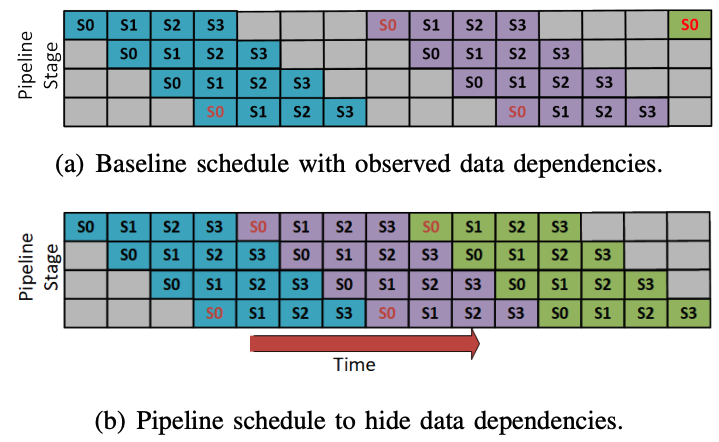
\includegraphics[width=0.6\linewidth]{./images/pipeline-schedule-deep-speed-inference.png}
        \caption{A pipeline parallel schedule for generating the first three tokens for four sequences $S0$ to $S3$.}
        }
    \end{figure}
\end{frame}


\begin{frame}{DeepSpeed Inference: Inference on Many GPU System: II}
    \begin{figure}
        \centering{
        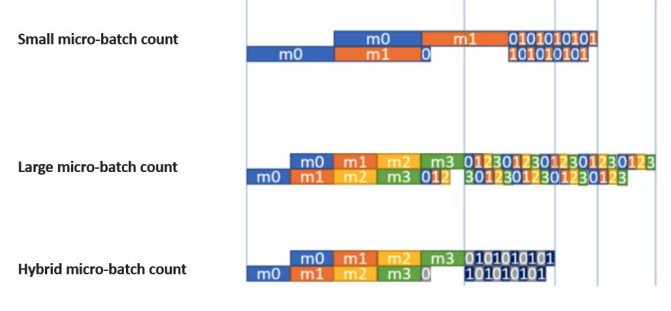
\includegraphics[width=0.7\linewidth]{./images/different-batch-size-in-pipeline-parallelism.png}
        \caption{Different micro-batch for prompt-processing and token-generation.}
        }
    \end{figure}
    \scriptsize{
    \begin{itemize}
        \item Suppose there are $P$ pipeline stage, it is necessary to have $P$ micro-batch to utilize all of the pipeline stages.
        \item The prompt processing stage has a large batch size that can saturate the GPU compute. macro-batches only affacts pipeline bubbles but not GPU execution time.
        \item The next token generation stage has a very small batch size, the performance is entirely bounded by reading weights. macro-batches number affacts execution time.
        \item \textbf{Solution}: \hl{large micro-batch count in prompt-processing and small micro-batch count in token generation}.
    \end{itemize}
    }
\end{frame}